%-------------------------------------------------------------------------------
% usr_file
%-------------------------------------------------------------------------------
%
% \file        usr_file.tex
% \library     Documents
% \author      Chris Ahlstrom
% \date        2015-08-31
% \update      2020-12-07
% \version     $Revision$
% \license     $XPC_GPL_LICENSE$
%
%     Provides the usr_file.
%
%-------------------------------------------------------------------------------

\section{Seq66 'usr' Configuration File}
\label{sec:usr_file}

   There are many \textsl{Seq66} configuration files:
   \texttt{qseq66.rc}
   \texttt{qseq66.usr},
   \texttt{qseq66.mutes},
   \texttt{qseq66.drums}, and
   \texttt{qseq66.playlist}.

%  See \sectionref{sec:rc_file}; it describes the 'rc' file.
%  It is a bit different in how it is handled.

   This section describes the \textsl{Seq66} 'usr' (or "user") file.
   The \textsl{Seq66} 'usr'
   configuration file provides a way to give more
   informative names to the MIDI busses, MIDI channels, and MIDI controllers of
   a given system setup.  This configuration overrides the default values
   of the \textbf{Event} drop-down list and menu items in the Pattern editor,
   and make them reflect the names of the MIDI Control (CC) values of one's
   devices.

   In \textsl{Seq66} it, also includes some items that affect the
   user-interface's look, and many other new configuration items.
   At some point we will likely split this file into another configuration file
   ("qseq66.ui"?)

   \index{usr!-u}
   \index{usr!--user-save}
   Unlike the 'rc' file, the 'usr' file is \textsl{not} written every time
   \textsl{Seq66} exits.  If the 'usr' files does not exist, one is
   created, but it is normally not overwritten thereafter.  To
   cause it to be overwritten at exit, run \textsl{Seq66} with the
   \texttt{-u} or \texttt{--user-save} option:

   \begin{verbatim}
      $ seq66 --user-save
   \end{verbatim}

   This option is recommended when one installs a new version of
   \textsl{Seq66}, which might add new options to the 'usr' file.
   See \sectionref{sec:man_page}; it discusses more options involving the
   'usr' file.

   Another difference between the 'rc' file and the 'usr' file is that
   the 'usr' file currently has no graphical user-interface dialog to
   configure the 'usr' settings.  One has to edit the file manually.
   There are a few items that can be tweaked in the \textsl{Seq66} application, and
   if they are modified, the user-save flag is turned on.

   By default, the list of MIDI devices that \textsl{Seq66} shows depends
   on one's system setup and whether the manual-port option is specified
   or not.  Here's our system, with the
   the \texttt{[manual-port]} option turned off, shown in a
   composite view with all menus one can look at for MIDI settings:

\begin{figure}[H]
   \centering 
   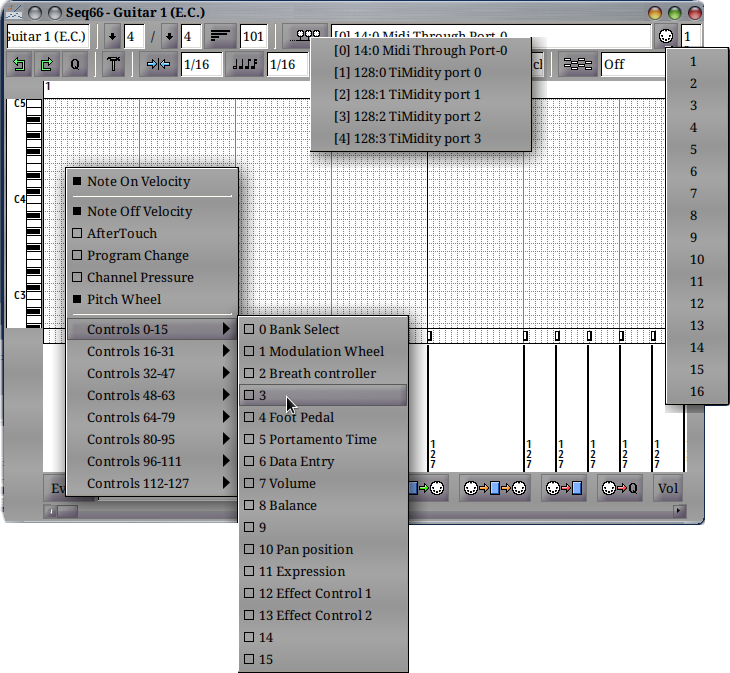
\includegraphics[scale=0.65]{usr/manual-0-buss-dropdown.png}
   \caption{Seq66 Composite View of Native Devices}
   \label{fig:manual_0_buss_dropdown}
\end{figure}

   At the top center, the dropdown menu contains the MIDI busses/ports
   supported by this computer.  At right, the MIDI channel shows
   the channels numbers that can be picked for buss 0.  At bottom left, we see
   the default controller values that \textsl{Seq66} includes.  We have
   no idea if these correspond to any controllers that the selected MIDI buss
   supports.  We \textsl{can} use this dropdown to see if any such controller
   events are in the loaded MIDI file, of course; a solid black square
   indicates that such an event was found in the pattern.

   To change the defaults, we can create a 'usr' file to set them up.
   The discussion here relies on the reader opening the file
   \texttt{sample.usr}, which is included in the shared \texttt{data/samples}
   directory provided once \textsl{Seq66} is installed.

   Assume we have 3 MIDI "buss" devices hooked to our system:
   two Model "2x2" MIDI port devices, and an old PCR-30 MIDI controller
   keyboard.  Let's number them:

   \begin{enumerate}
      \item Model 2x2 A
      \item Model 2x2 B
      \item PCR-30
   \end{enumerate}

   Then assume that we have nine different MIDI instruments in our kit.
   Let's number them, too:

   \begin{enumerate}
      \item Waldorf Micro Q
      \item SuperNova
      \item DrumStation
      \item TX81Z
      \item WaveStation
      \item ESI-2000
      \item ES-1
      \item ER-1
      \item TB-303
   \end{enumerate}

   The \textsl{Waldorf Micro Q},
   the \textsl{SuperNova},
   and the \textsl{DrumStation} all have a large
   number of special MIDI controller values for modifying the sound they
   produce.
   The \textsl{DrumStation} accepts MIDI controllers that change various
   features of the sound of each type of drum it supports.

   The buss devices can be configured to route certain
   MIDI channels to certain MIDI devices.  Assume we have them
   set up this way:

   \begin{enumerate}
      \item Bus 0: Model 2x2 A
      \begin{itemize}
         \item SuperNova: channels 1 to 8
         \item TX81Z: channels 9 to 11
         \item Waldorf Micro Q: channels 12 to 15
         \item DrumStation: channel 16
      \end{itemize}
      \item Bus 1: Model 2x2 B
      \begin{itemize}
         \item WaveStation: channels 1 to 4
         \item ESI-2000: channels 5 to 14
         \item ES-1: channel 15
         \item ER-1: channel 16
      \end{itemize}
      \item Bus 2: PCR-30
      \begin{itemize}
         \item TB-303: channel 1
      \end{itemize}
   \end{enumerate}

   We use the \textbf{'usr' configuration file}.
   to show these items with the proper
   names associated with each device, channel, and controller value

   \index{seq66.usr}
   The \textsl{Seq24} configuration file was called
   \texttt{.seq24usr}, and it was stored in the user's \texttt{\$HOME}
   directory.
   \textsl{Seq66} uses a new file-name
   to take its place.
   After one runs \textsl{Seq66} for the first time (or after deleting
   the configuration files), it will generate a
   \texttt{seq66.usr} file in one's HOME directory:

   \begin{verbatim}
      /home/user/.config/seq66/seq66.usr
   \end{verbatim}

   It allows you to give an alias to 
   each MIDI bus, MIDI channel, and MIDI control 
   codes, per channel.
   The process for setting up the 'usr' file is to:

   \begin{enumber}
      \item Define one or more MIDI busses, the name of each, and what
         instruments are on which channels.  Each buss is configured in a
         section of the form "\texttt{[user-midi-bus-X]}", where "X" ranges
         from 0 on up.  Each buss then defines up to 16 channel entries.
         Each entry includes the channel number and the number of a
         section in the user-instrument section described next.
      \item Define all of the instruments and their controller
         names, if they have them.  Each instrument is configured in a
         section of the form "\texttt{[user-instrument-X]}", where "X"
         ranges from 0 on up.  Up to 128 controllers can be defined.
   \end{enumber}

   Let's walk through the structure of this setup, since it is a little bit
   tricky.  Here is a diagram of the relationships between the buss definitions
   and instrument definitions:

\begin{figure}[H]
   \centering 
   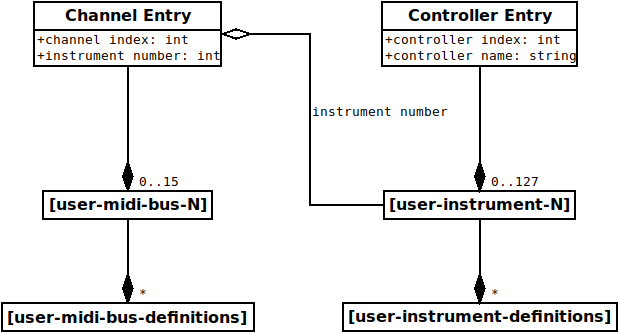
\includegraphics[scale=0.50]{usr/user-busses-and-instruments.png}
   \caption{Busses and Instruments in the 'usr' File}
   \label{fig:manual_user_busses_and_instruments}
\end{figure}

   The first section in the 'usr' file (after \texttt{[comments]})
   is \texttt{[user-midi-bus-definitions]}.  The solid diamond link, with the
   "*" marker, indicates that this section contains an arbitrary number ("*")
   of \texttt{[user-midi-bus-N]} sections, where "N" ranges from 0 on upward.
   These correspond to the MIDI busses expected to be in the system, ignoring
   the ALSA "announce" buss.

   Each of the busses contains 16 (0 to 15) channel entries.
   These channels are referred to as "instrument numbers", and are
   represented as and linked to "instruments" in the
   \texttt{[user-instrument-definitions]} section.  Each instrument contains up
   to 128 controller values; these controller values are available in the
   \textbf{Event} button in the Pattern Editor, and their names are shown.

   So, each instrument is setup as a "channel" in a particular "buss".
   In the Pattern Editor, when a particular buss and channel is selected,
   the \textbf{Event} menu entries should match the controller entries set up
   in the 'usr' file.

   The list of devices and channels shown earlier
   can be seen in the \textsl{Seq66} sample file
   \texttt{data/samples/sample.usr}.
   Deducting 1 from each device number and channel number (so that numbering
   starts from 0), and consulting the device manuals to determine the
   controller values supported, one can assemble a 'usr' configuration file
   that makes the setup visible in \textsl{Seq66}.

   Peruse the next couple of sections to understand a bit about the format of
   this file, following along in the sample 'usr' file.
   Once satisfied, go to
   \sectionref{subsec:usr_file_midi_bus_results}, and 
   see what it all looks like.

\subsection{'usr' File / MIDI Bus Definitions}
\label{subsec:usr_file_midi_bus_definitions}

   \index{usr!user-midi-bus-definitions}
   \index{[user-midi-bus-definitions]}
   This section begins with an
   "INI" group marker \texttt{[user-midi-bus-definitions]}.
   It defines the number of user busses that will be configured in this file.

   \begin{verbatim}
      [user-midi-bus-definitions]
      3     # number of user-defined MIDI busses
   \end{verbatim}

   \index{usr!user-midi-bus-n}
   \index{[user-midi-bus-n]}
   This means that the 'usr' file will have three MIDI buss
   sections: [user-midi-bus-0], [user-midi-bus-1], and [user-midi-bus-2].
   Here's is an example of one such section:

   \begin{verbatim}
      [user-midi-bus-0]
      2x2 A (SuperNova,Q,TX81Z,DrumStation)
      16
      0 1
      1 1      # Instrument #1 of the [user-instrument-definitions] section
      2 1
      . . .
      8 3      # Instrument #3 of the [user-instrument-definitions] section
      9 3
      10 3
      11 0     # Instrument #0 of the [user-instrument-definitions] section
      12 0     # This is the Waldorf Micro Q device defined below
      13 0
      14 0
      15 2     # Instrument #2 of the [user-instrument-definitions] section
   \end{verbatim}

   Here's an example of one that needs only one override:

   \begin{verbatim}
      [user-midi-bus-2]
      PCR-30 (303)
      1
      0 8
      # The rest default to -1... General MIDI
   \end{verbatim}

   These user-instrument entries can be quickly disabled by changing
   the count values to 0.
   These instrument-definition
   sections are read from the 'usr' configuration file only if
   the \texttt{--reveal-ports} option is \textsl{off} ("0");
   this option can also be specified in the
   \texttt{[reveal-ports]} section of the 'rc' file,
   see \sectionref{subsec:rc_file_reveal_ports}.
   Otherwise, the actual port names reported by ALSA are shown.
   The \texttt{user-midi-bus-definitions} and \texttt{user-midi-bus-N} sections
   can be misleading if one wants to have access to the
   actual ALSA ports that exist on the system.

   Try these combinations of options to see what they look like:

   \begin(itemize)
      \item Clocks View, -m (--manual-ports)
      \item Clocks View, -m (--manual-ports) and -R (--hide-ports)
      \item Clocks View, -r (--reveal-ports)
      \item Clocks View, -R (--hide-ports)
      \item Inputs View, -m (--manual-ports)
      \item Inputs View, -r (--reveal-ports)
      \item Inputs View, -R (--hide-ports)
   \end(itemize)

\iffalse

   The following figures show the results of various settings with an
   active 'usr' file.  They have been clipped to save space.

\begin{figure}[H]
   \centering 
   \includegraphics[scale=0.50]{user/seq66-clock-m.png}
   \caption{Clocks View, -m (--manual-ports)}
   \label{fig:clock_m}
\end{figure}

   Above, the virtual (manual) output ports are shown just as created by
   \textsl{Seq66}.
   The \texttt{--reveal-ports} option is \textsl{off} here.

\begin{figure}[H]
   \centering 
   \includegraphics[scale=0.50]{user/seq66-input-m.png}
   \caption{Inputs View with -m (--manual-ports) Option}
   \label{fig:input_m}
\end{figure}

   Above, the single virtual (manual) input port is shown just as created by
   \textsl{Seq66}.
   Again, the \texttt{--reveal-ports} option is \textsl{off} here.

\begin{figure}[H]
   \centering 
   \includegraphics[scale=0.50]{user/seq66-clock-m-R.png}
   \caption{Clocks View, -m (--manual-ports) and -R (--hide-ports)}
   \label{fig:clock_m_R}
\end{figure}

   Above, by adding the "hide" ports option, the system port labels are
   replaced by the labels from the 'usr' file.

\begin{figure}[H]
   \centering 
   \includegraphics[scale=0.50]{user/seq66-clock-r.png}
   \caption{Clocks View, -r (--reveal-ports)}
   \label{fig:clock_r}
\end{figure}

   Above, the "reveal" ports option overrides the device names given in the
   'usr' file, so that the native system names of the output ports are shown.

\begin{figure}[H]
   \centering 
   \includegraphics[scale=0.50]{user/seq66-input-r.png}
   \caption{Inputs View with -r (--reveal-ports) Option}
   \label{fig:input_r}
\end{figure}

   Above, the "reveal" ports option overrides the device names given in the
   'usr' file, so that the native system names of the input ports are shown.
   However, \textsl{Seq66} no longer overrides the
   names of the input ports via the 'usr' file.  This is done to
   save some trouble in displaying the input port names, which are shown
   only in this dialog.  We may consider offering a separate override section
   for the input ports in the future.

\begin{figure}[H]
   \centering 
   \includegraphics[scale=0.50]{user/seq66-clock-R.png}
   \caption{Clocks View with -R (--hide-ports) Option}
   \label{fig:clock_R}
\end{figure}

   The figure above shows how hiding the system port names shows the names
   defined in the 'usr' file.  But notice that the actual port names are shown
   in square brackets, for reference.

\begin{figure}[H]
   \centering 
   \includegraphics[scale=0.50]{user/seq66-input-R.png}
   \caption{Inputs View with -R (--hide-ports) Option}
   \label{fig:input_R}
\end{figure}

   Although the "hide" ports option is specified above, this view is
   currently also the normal view of the input ports, even with device names
   defined in the 'usr' file.
   At this time, there's no real need to show the user-instrument names
   on the input port.  If there turns out to be such a need, the definitions
   would likely need to be different from the definitions for the output ports.
   Another complexity is the possible existence, under ALSA, of the
   \texttt{system:announce} port.

\fi

\subsection{'usr' File / MIDI Instrument Definitions}
\label{subsec:usr_file_midi_instrument_definitions}

   \index{usr!user-instrument-definitions}
   \index{[user-instrument-definitions]}
   This section begins with an
   "INI" group marker \texttt{[user-instrument-definitions]}.
   It defines the number of user instruments that will be configured in this
   file.  This section defines characteristics, such as
   the meanings of MIDI controller values, of the instruments themselves,
   not the MIDI busses to which they attached.

   \begin{verbatim}
      [user-instrument-definitions]
      9     # number of user instrument
   \end{verbatim}

   \index{usr!user-instrument-n}
   \index{[user-instrument-n]}
   So this 'usr' file will define 9 instruments.  We provide only one section
   as an example.  Note that items without text default to the values
   prescribed by the General MIDI (GM) specification.

   \begin{verbatim}
      [user-instrument-0]
      Waldorf Micro Q                     # name of instrument
      128                                 # number of MIDI controllers
      0                                   # first controller value, unnamed
      1 Modulation Wheel
      2 Breath Control
      3 
      4 Foot Control
         . . .
      119
      120 All Sound Off (0)
      121 Reset All Controllers (0)
      122 Local Control (0-127) (Off,On)
      123 All Notes Off (0)
      124                                 # defaults to GM
      125 Unsupported
      126 Unsupported
      127                                 # defaults to GM
   \end{verbatim}

   Note the unnamed control numbers above.
   An unnamed control number might be an unsupported control number.
   It is termed to be "inactive".  In this case, the \textbf{Event} menu of
   the Pattern editor will show the default name of this controller.
   Again, though, the function denoted by this name might not be supported by
   the device.  In that case, it might be better to call it "Unsupported".
   See the examples above.

\subsection{'usr' File / User Interface Settings}
\label{subsec:usr_file_user_interface_settings}

   \index{usr!user-interface-settings}
   \index{[user-interface-settings]}
   This section, new to \textsl{Seq66}, begins with an
   "INI" group marker \texttt{[user-interface-settings]}.

   It provides for a feature we will hopefully be able to complete some day:
   the complete specificition of the appearance of the user-interface.
   There is plenty of room to change the appearance of
   \textsl{Seq66} already!  Please try the settings and see what looks good.
   Refer to either the sample file or the file generated when \textsl{Seq66} first
   runs.

   \index{usr!grid-style}
   \begin{verbatim}
      [user-interface-settings]
      1       # grid_style
   \end{verbatim}

   \index{usr!grid-brackets}
   \begin{verbatim}
      2       # grid_brackets
   \end{verbatim}

   \index{usr!mainwnd-rows}
   \index{variset}
   \begin{verbatim}
      4       # mainwnd_rows
   \end{verbatim}

   \index{usr!mainwnd-cols}
   \index{variset}
   \begin{verbatim}
      8       # mainwnd_cols
   \end{verbatim}

   \index{usr!max-sets}
   \begin{verbatim}
      32      # max_sets
   \end{verbatim}

   \index{usr!mainwid-border}
   \begin{verbatim}
      0      # mainwid_border
   \end{verbatim}

   \index{usr!mainwid-spacing}
   \begin{verbatim}
      2      # mainwid_spacing
   \end{verbatim}

   \index{usr!control-height}
   \begin{verbatim}
      0      # control_height
   \end{verbatim}

   \index{usr!zoom}
   \begin{verbatim}
      2      # zoom
   \end{verbatim}

   \index{usr!global-seq-feature}
   \begin{verbatim}
      1      # global_seq_feature
   \end{verbatim}

   \index{usr!use-new-font}
   \begin{verbatim}
      1      # use_new_font
   \end{verbatim}

   \index{usr!allow-two-perfedits}
   \begin{verbatim}
      1      # allow_two_perfedits
   \end{verbatim}

   \index{usr!perf-h-page-increment}
   \begin{verbatim}
      4      # perf_h_page_increment
   \end{verbatim}

   \index{usr!perf-v-page-increment}
   \begin{verbatim}
      8      # perf_v_page_increment
   \end{verbatim}

   \index{usr!progress-bar-colored}
   \begin{verbatim}
      6      # progress_bar_colored
   \end{verbatim}

   \index{usr!progress-bar-thick}
   \begin{verbatim}
      1      # progress_bar_thick
   \end{verbatim}

   \index{usr!inverse-colors}
   \begin{verbatim}
      0      # inverse_colors
   \end{verbatim}

   \index{usr!window-redraw-rate}
   \begin{verbatim}
      40     # window_redraw_rate
   \end{verbatim}

   \index{usr!use-more-icons}
   \begin{verbatim}
      0      # use_more_icons (currently affects only main window)
   \end{verbatim}

   \index{usr!block-columns}
   \begin{verbatim}
      2      # block_columns (number of columns of set blocks/wids)
   \end{verbatim}

   \index{usr!block-independent}
   \begin{verbatim}
      1      # block_independent (separate set spinner for blocks/wids)
   \end{verbatim}

   Note that the window-redraw rate option is meant more for experimentation
   than anything else.  It probably doesn't affect CPU usage much, but might
   provide a smoother-running cursor on some systems.

\subsection{'usr' File / User MIDI Settings}
\label{subsec:usr_file_user_midi_settings}

   \index{[user-midi-settings]}
   This section begins with an
   "INI" group marker \texttt{[user-midi-settings]}.
   It supports files with different PPQN, and and allows one to specify the
   global defaults for tempo, beats per measure, and so on.

   \index{usr!midi-ppqn}
   \begin{verbatim}
      [user-midi-settings]
      192     # midi_ppqn
   \end{verbatim}

   \index{usr!midi-beats-per-measure}
   \begin{verbatim}
      4       # midi_beats_per_measure/bar
   \end{verbatim}

   \index{usr!midi-beats-per-minute}
   \begin{verbatim}
      120     # midi_beats_per_minute
   \end{verbatim}

   \index{usr!midi-beat-width}
   \begin{verbatim}
      4       # midi_beat_width
   \end{verbatim}

   \index{usr!midi-buss-override}
   \begin{verbatim}
      -1     # midi_buss_override
   \end{verbatim}

   \index{usr!velocity-override}
   \begin{verbatim}
      80     # velocity_override (-1 = 'Free')
   \end{verbatim}

   \index{usr!bpm-precision}
   \begin{verbatim}
      1      # bpm_precision
   \end{verbatim}

   \index{usr!bpm-step-increment}
   \begin{verbatim}
      0.1    # bpm_step_increment
   \end{verbatim}

   \index{usr!bpm-page-increment}
   \begin{verbatim}
      5.0    # bpm_page_increment
   \end{verbatim}

   \index{usr!midi-bpm-minimum}
   \begin{verbatim}
		0       # midi_bpm_minimum
   \end{verbatim}

   \index{usr!midi-bpm-maximum}
   \begin{verbatim}
		360       # midi_bpm_maximum
   \end{verbatim}

   \index{usr!velocity-override}
      The \texttt{velocity-override} option fixes a long standing (from
      \textsl{Seq24}) bug where the actual incoming note velocity was always
      replaced by a hard-wired value.

   \index{usr!bpm-step-increment}
   \index{usr!bpm-page-increment}
      The \texttt{bpm-precision}, \texttt{bpm-step-increment}, and
      \texttt{bpm-page-increment} values allow more precise control over tempo,
      which makes it easier to match the tempo of external music sources.  Note
      that the step-increment is used by the up/down arrow buttons, the up/down
      arrow keys, and the MIDI BPM control values.  The page-increment is used
      if the BPM field has focus and the Page-Up/Page-Down keys are pressed,
      and new MIDI control values have been added to support coarse MIDI
      control of tempo.

   \index{usr!midi-bpm-minimum}
   \index{usr!midi-bpm-maximum}
		The \texttt{midi-bpm-minimum} and \texttt{midi-bpm-maximum} settings
		are used in scaling the display of Tempo events.
      By adjusting these values, one can more easily see the variations in
      tempo.  In a main window pattern slot, or in the song editor tempo track,
      this range is scaled to the full range of note values, 0 to 127.
      Generally, one wants to select a range that keeps the main tempo line at
      the middle height of the pattern display.

   To obtain these new settings, remember to backup the existing
   \textsl{seq66.usr}, then run \textsl{Seq66} with the
   \texttt{--user-save} option, and then do a "diff" on the new file and the
   original to merge any old values that need to be preserved.  Then make any
   further tweaks to the new values.

\subsection{'usr' File / User Options}
\label{subsec:usr_file_user_options}

   \index{[user-options]}
   This section begins with an
   "INI" group marker \texttt{[user-options]}.
   It provides for additional options keyed by the
   \texttt{-o}/\texttt{--option} options.
   This group of options serves to expand the options that are available, since
   \textsl{Seq66} is  running out of single-character options.
   This group of options are shown below.

   \index{usr!option-daemonize}
   \begin{verbatim}
		0       # option_daemonize
   \end{verbatim}

   If this option is not used when running \texttt{seq66cli}, then the
   application stays in the console window and dumps informational output to
   it.  If this option is in force, then the only way to affect
   \texttt{seq66cli} is to send a signal (e.g. SIGKILL) to it, or use
   MIDI control.

   \index{usr!option-logfile}
   \begin{verbatim}
      "seq66.log"
   \end{verbatim}

   This log-file is written to the same directory as the 'rc' and 'usr' files.
   If this file-name is empty, then a valid file-name must be specified
   in the "--option log=filename.log" option.  Note that this file
   is always written to the \textsl{Seq66} configuration directory.

\subsection{'usr' File / Device and Control Names}
\label{subsec:usr_file_midi_bus_results}

   Okay, now we have this file copied to our home directory:

   \begin{verbatim}
      /home/user/.config/seq66/seq66.usr
   \end{verbatim}

   If we'd already run \textsl{Seq66} at least once, we'd have
   overwritten the skeleton sample file that \textsl{Seq66}
   writes by default.  We now have a full-fledged 'usr' file.

   However, because we don't actually have all that equipment (we got the
   example from the Web, for cryin' out loud), let's see what we end up with
   when we run \textsl{Seq66} this time and show the pattern editor
   settings:

\begin{figure}[H]
   \centering 
   \includegraphics[scale=0.65]{usr/manual-0-userfile-buss-dropdown.png}
   \caption{Seq66 Composite View of Non-Native Devices}
   \label{fig:manual_0_userfile_buss_dropdown}
\end{figure}

   Compare that diagram to \figureref{fig:manual_0_buss_dropdown}.
   If the original figure, we saw the 5 native busses (ports) on our system,
   their bare-bones channel numbers, and the default controller values.  In
   this new figure, we see the three buss devices (ports), plus the two
   Timidity ports.  If we stopped the Timidity service, these would go away.

   Look at the selected buss, "[0]".  It's 16 channels are now associated with
   the devices to which the channels have been assigned.
   Thus, when we have a new pattern we've created in \textsl{Seq66},
   we can assign it to exactly the buss and device we want.

   If we don't have port-mappers installed, and thus have only one playback
   device plugged into the buss, we can still create a setup that
   shows the device and a specific program setup.  Doing so would be tedious,
   but perhaps there's some automated way to do it?
   Lastly, note the following figure.

\begin{figure}[H]
   \centering 
   \includegraphics[scale=0.65]{usr/manual-0-userfile-seq-buss-dropdowns.png}
   \caption{The MIDI Bus Menu for a Specific Pattern}
   \label{fig:manual_0_userfile_seq_buss_dropdown}
\end{figure}

   This figure shows that we can also select the desired port and channel
   directly from the main window.
   There's more to the 'usr' configuration file than we've exposed here.
%  but finding more information about this file has proven a bit tricky.

%  Sometime we would like to create a 'usr' that sets up the
%  \textsl{Yoshimi} 1.3.5+ software synthesizer as a device and instrument.

%-------------------------------------------------------------------------------
% vim: ts=3 sw=3 et ft=tex
%-------------------------------------------------------------------------------
